\chapter{State Spaces}
\label{chap:quicksand}

In this chapter, I will present a new algorithm for model checkers to automatically choose which preemption points to use to test reasonably-sized state spaces.
This is the first of the three projects I am proposing for this thesis, and has already been published at OOPSLA 2016 \cite{quicksand}.
The thesis will largely restate the paper, and also go into more detail on some ideas which didn't make it into the paper, such as measuring the variance in each experimental data series.
Here in the proposal I will simply summarize the content of the paper.

\section{Motivation}
\label{sec:qs-motivation}

This project is motivated by my experience contributing to Parrot \cite{parrot},
a (partially) determinizing runtime for multithreaded programs which allowed some nondeterminism in performance-critical sections to achieve high performance.
We combined Parrot with dBug \cite{dbug-ssv}, a model checker, to check the correctness of the nondeterministic sections of programs which remained.
Unfortunately, dBug was able to finish a state space for fewer than half of these programs in our evaluation in a 24-hour time limit,
even after the reduction Parrot provided.
In that project, our model checker was limited to a fixed set of preemption points;
in other words, it would always test different programs with the same granularity of thread interleavings.
Consequently, the resulting completion time for each test would vary wildly,
unpredictably falling on one side or the other of our arbitrary time limit.

I argue that this is the wrong usage model for model checkers to present to users who wish to test for concurrency bugs.
Users want concrete bug reports (obviously), or in absence of those, they want some assurance of the program's correctness.
However, users do not live in a $\infty$-sized fantasy land \cite{vargomax},
and are generally willing to wait only for some fixed finite time.
If full verification of all possible interleavings is not possible within that time,
a {\em partial verification} guarantee for some smaller state spaces is better than an ``I don't know'' verdict for one single state space.

%%%%%%%%%%%%%%%%%%%%%%%%%%%%%%%%%%%%%%%%%%%%%%%%%%%%%%%%%%%%%%%%%%%%%%%%%%%%%%%%

\section{Design}

Hence, I propose a more user-friendly framework for model checking, in which many different state spaces are tested,
and higher priority is given to state spaces which appear possible to complete before the user's patience runs out or their project is due.
At the heart of this framework is an algorithm I call {\bf Iterative Deepening},
by analogy with the eponymous technique in chess artificial intelligence \cite{iterative-deepening-chess-ai}.
In both chess and model checking, Iterative Deepening makes progressively ``deeper'' searches of an exponentially-sized state space,
repeatedly increasing the size of a subset state space to be explored,
until a prescribed time limit is exceeded.
While in chess, the size bound is determined by a single depth parameter,
the size of model checking state spaces is determined by any number of different combinations of preemption points being enabled or disabled.

{\bf Quicksand.}
I have built a wrapper program, called Quicksand, which manages the execution of multiple simultaneous Landslide instances.
Quicksand relies on state space estimation \cite{estimation} to decide at runtime how to prioritize these jobs.
Landslide can provide these estimates to a reasonable accuracy before actually testing a large fraction of interleavings for a given state space.
Quicksand seeks to maximize completed state spaces,
as each one serves as a guarantee that all interleavings possible with its preemption points were tested.
Moreover, because Iterative Deepening treats the set of preemption points as mutable,
it can add new preemption points reactively based on any runtime analysis.
Landslide begins with a statically-coded set of synchronization API preemption points (such as used by dBug \cite{dbug-ssv}),
and during testing, runs a dynamic data-race analysis \cite{hybriddatarace,tsan,ifrit} to identify new candidate preemption points.

\newcommand\PendingJobs{\ensuremath{\mathcal{P}}}
\newcommand\SuspendedJobs{\ensuremath{\mathcal{S}}}
\newcommand\GetETA[1]{ETA(#1)}
\newcommand\GetPPSet[1]{PPSet(#1)}

{\bf Iterative Deepening.}
With a limited CPU budget, Quicksand must avoid running tests that are likely to be fruitless.
Hence, it separates the available preemption point sets into a set of {\em suspended} jobs (partially-explored state spaces with high ETAs),
and a set of {\em pending} jobs (untested ones with unknown ETAs).
When Landslide reports an ETA exceeding the time limit,
Quicksand compares with other pending and suspended jobs to find another one more likely to complete in time.
The Iterative Deepening algorithm implements this comparison, presented formally in Algorithm~\ref{alg:shouldworkblock}.
Its main feature is understanding that when one Landslide instance is testing a superset of preemption points compared to another, the state space is correspondingly guaranteed to contain a superset of possible thread interleavings.
%This allows it to extend estimation information for too-large state spaces to even larger state spaces
%that if \GetPPSet{$j_1$} $\subset$ \GetPPSet{$j_2$},
%and $j_1$ is suspended,
%then $j_2$'s state space is guaranteed to be strictly larger, so $j_2$ will take at least as long.
%Hence we should avoid testing $j_2$ unless $j_1$ is later resumed and its ETA improves after further execution. %over time.
%%reveals that it might finish in time after all.
%Similarly, whenever a job finds a bug, we cancel all pending superset jobs, as they might find only the same bug.

\begin{algorithm}[h]
        \SetKwInOut{Input}{Input}
        %\textbf{Function} GetBestJob($j_0$, PendingJobs, SuspendedJobs): \\
        \Input{$j_0$, the currently-running job}
        %\Input{$eta$, $j_0$'s predicted completion time}
        \Input{\PendingJobs, the list of pending jobs, sorted by decreasing heuristic priority}
        \Input{\SuspendedJobs, the list of already-suspended jobs, sorted by increasing ETA}
        \Input{$T$, the remaining time in the CPU budget}
        \If{\GetETA{$j_0$} $<$ HeuristicETAFactor $\times$ $T$}{
                return $j_0$ // Common case: job is expected to finish.
        }
        \ForEach{job $j_P \in$ \PendingJobs}{
                // Don't run a pending job if a subset of it is already suspended; its ETA would be at least as bad. \\
                \If {$\forall j_S \in$ \SuspendedJobs, \GetPPSet{$j_S$} $\not\subset$ \GetPPSet{$j_P$}}{
                        return $j_P$
                }
        }
        %// no pending jobs; maybe resume a suspended job \\
        \ForEach{job $j_S \in$ \SuspendedJobs}{
                \If{\GetPPSet{$j_0$} $\not\subset$ \GetPPSet{$j_S$}
                        $\land$
                        \GetETA{$j_0$} $>$ \GetETA{$j_S$}}{
                        // If a subset of $j_S$ is also suspended, don't run the larger one first. \\
                        \If{$\forall j_{S2} \in$ \SuspendedJobs, \GetPPSet{$j_{S2}$} $\not\subset$ \GetPPSet{$j_S$}}{
                                return $j_S$
                        }
                }
        }
        return $j_0$ // \GetETA{$j_0$} was bad, but no other $j$ was better.
        \caption{Suspending exploration of a state space in favour of a potentially smaller one.}
        \label{alg:shouldworkblock}
\end{algorithm}

\newcommand\AllJobs{\ensuremath{\mathcal{J}}}
\begin{algorithm}[h]
        \SetKwInOut{Input}{Input}
        \Input{$j_0$, the currently-running job}
        \Input{\AllJobs, the set of all existing (or completed) jobs}
        \Input{$\alpha$, an instruction reported by the MC as part of a racing access pair}
        \If{$\forall j \in \AllJobs,$
        \GetPPSet{$j_0$} $\cup$ $\alpha$
        $\not\subseteq$
        \GetPPSet{$j$}
        }{
                AddNewJob(\GetPPSet{$j_0$} $\cup$ $\alpha$, HeuristicPriority($\alpha$)) \\
        }
        \If{$\forall j \in \AllJobs,$ \GetPPSet{$j$} $\neq \{yield, \alpha\}$}{
                AddNewJob($\{yield, \alpha\}$, HeuristicPriority($\alpha$))
        }
        \caption{Adding new jobs with data-race PPs.}
        \label{alg:handledatarace}
\end{algorithm}

{\bf Data-race preemption points.}
As mentioned, runtime data race analysis produces new potential sites at which preempting the program may produce new behaviour.
With Iterative Deepening, this is a simple matter of creating a new state space with an additional preemption point enabled on the racing instructions by each thread, shown formally in Algorithm~\ref{alg:handledatarace}.
The new state spaces may expose a failure, in which case Landslide reports a data-race bug,
or complete successfully, indicating a benign or false-positive data race.
They may also uncover a new data-race candidate entirely, %in some alternate interleaving,
in which case Quicksand iteratively advances to a superset state space containing PPs for both racing access pairs.
Being constrained by a CPU budget,
time may run out before completing a data race's associated state space,
in which case Quicksand reports a potential false positive that the user must handle.

%%%%%%%%%%%%%%%%%%%%%%%%%%%%%%%%%%%%%%%%%%%%%%%%%%%%%%%%%%%%%%%%%%%%%%%%%%%%%%%%

\section{Verification}

\subsection{Convergence of Iterative Deepening}
When the a test's state spaces are small enough that Quicksand can exhaustively check all of them within a given CPU budget,
the resulting verification claim turns out to be equivalent to a na\"{i}model checker which preempts on every memory access.
In this way, the Iterative Deepening algorithm provides the ``best of both worlds'' for the tradeoff mentioned in Section~\ref{sec:qs-motivation}:
when tests are too large, Quicksand falls back on prioritization heuristics to find bugs quickly;
when tests are tractable, Quicksand's verification is equal to the strongest from any single-state-space technique.

The theorem statement is as follows:

\begin{theorem}[Convergence]
	If a bug can be exposed by any
thread interleaving possible by preempting on all instructions during a specific test, Iterative Deepening will eventually test an equivalent interleaving which exposes the same bug.
\end{theorem}

The proof is available at \cite{quicksand-soundness}.

\subsection{Pruning false-positive data-race candidates}
I have also proved a (somewhat less remarkable) theorem concerning the soundness of a new tactic for pruning certain types of false-positive data race candidates (under Limited HB).
A ``malloc-recycle'' false positive occurs when two threads seem to race on the same memory address, but only because the {\tt malloc}ed block containing that address was {\tt free}d and reallocated in between.
If the transitions of the two threads were reordered, the address collision would disappear and there would be no race.
The proof is available at \cite{quicksand-soundness}; the theorem statement is:

\begin{theorem}[Soundness of eliminating malloc-recycle candidates]
	If a malloc-recycle candidate is not a false positive,
	DPOR will test an alternate thread interleaving in which the
	accesses can race without fitting the malloc-recycle pattern.
\end{theorem}

%%%%%%%%%%%%%%%%%%%%%%%%%%%%%%%%%%%%%%%%%%%%%%%%%%%%%%%%%%%%%%%%%%%%%%%%%%%%%%%%

\section{Evaluation}

I evaluated Quicksand on the product of the following two questions: For an arbitrary fixed CPU budget...

\begin{itemize}
	\item ...does Quicksand find more bugs than a single-state-space (SSS-MC) approach...
	\item ...does Quicksand provide more total verifications than SSS-MC...
\end{itemize}
...where the SSS-MC control is configured to preempt...
\begin{itemize}
	\item ...on synchronization API boundaries only?
	\item ...on every single shared memory access?
\end{itemize}

I also conducted a separate experiment focused on the issue of {\em nondeterministic} data-races:
candidates that require model checking to expose in the first place, which would be
false-negatives during a single-execution analysis.

I also also ran several different configurations of Quicksand in each of these experiments,
alternately using Limited Happens-Before or Pure Happens-Before for its data-race analysis.
Both of these cases outperformed all the other cases of SSS-MC, so this was mostly useful for comparing the two techniques against each other.

\subsection{Setup and Test Suite}

The test suite for all these experiments was 157 student projects: 79 P2 thread libraries from CMU, and 78 Pintos kernels from Berkeley and the University of Chicago (Section~\ref{sec:overview-edu}).
I paired each submission with several test cases, 6 for each P2 and 3 for each Pintos.
In total there were 629 unique pairs of a test case and a student project, henceforth called simply ``tests''.
(Savvy mathematicians will note that doesn't quite add up -- some of the Pintoses were incomplete, and could only run 1 or 2 tests.)

For each of the 629 tests, I ran Quicksand and SSS-MC for 10 CPU-hours each in each of the configurations named above.
Quicksand, being inherently parallel, was given 10 CPUs for 1 wall-clock hour,
while SSS-MC control experiments were given 10 wall-clock hours on 1 CPU
(which is being charitable: comparing CPU-time gives the controls perfectly efficient hypothetical scaling from parallelization).

\subsection{Results}

The results are shown in Figure~\ref{fig:graphs}.
The first 3 graphs all plot a cumulative distribution of their respective achievements,
with elapsed time on the X-axis (as a log scale, to emphasize detail in the ``easy'' tests).
The captions largely explain each result.
To summarize, Quicksand outperforms the state-of-the-art on all metrics, excepting the impact of parallelization start-up overhead for very small CPU-time limits.
The Limited HB data-race strategy generally finds bugs faster when they exist,
but suffers on total verifications compared to Pure HB,
because of its false positives which create excess redundant state spaces for Landslide to check.

\begin{figure}[h]
	\begin{tabular}{cc}
		\begin{tabular}{p{0.48\textwidth}p{0.48\textwidth}}
			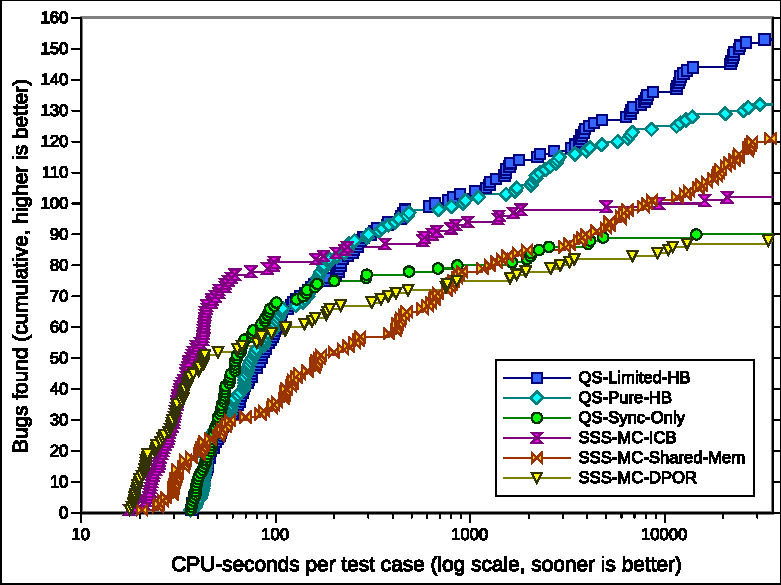
\includegraphics[width=0.48\textwidth]{dowefindbugsfaster-v2.pdf}
		&
			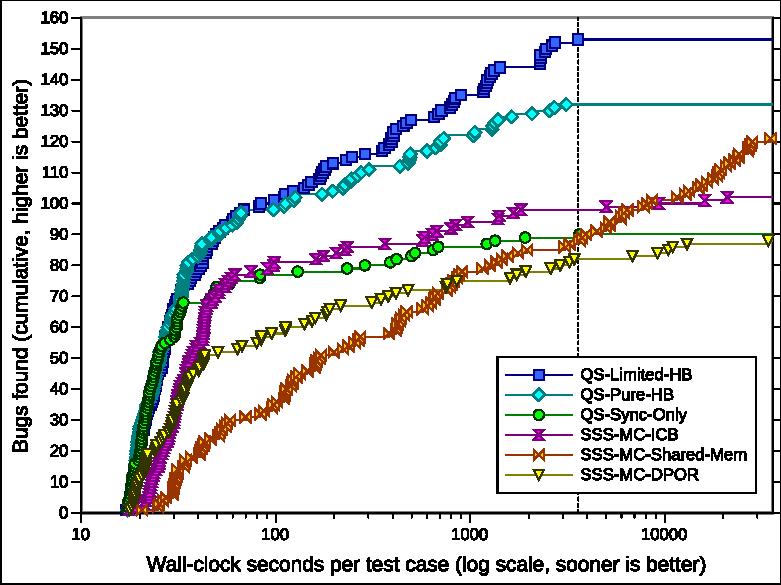
\includegraphics[width=0.48\textwidth]{dowefindbugsfaster-wallclock-v2.pdf}
		\\
			(a)
			Bugs found as a function of elapsed CPU time. After the break-even point at
			\textasciitilde{}200 seconds, Quicksand outperforms all control experiments.
		&
			(b)
			Bugs found by elapsed wall-clock time.
			This presentation emphasizes that the ``break-even'' point in (a)
			is just an artifact of parallelization start-up overhead.
			Quicksand is parallelized tenfold; the vertical line indicates its 1 hour limit.
		\\
			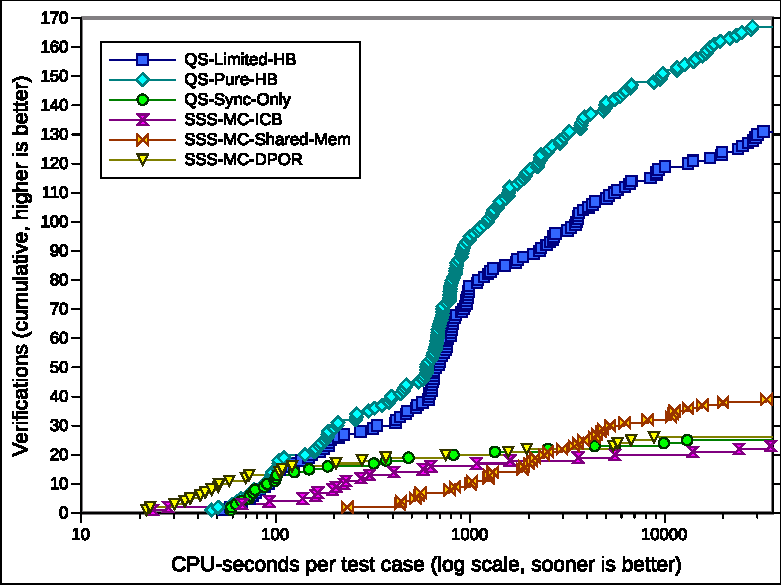
\includegraphics[width=0.48\textwidth]{totalverifs-v2.pdf}
		&
			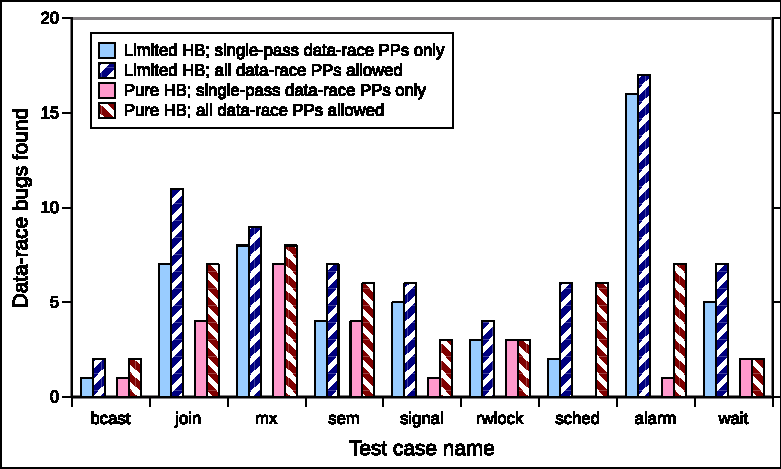
\includegraphics[width=0.48\textwidth]{nondets.pdf}
		\\
			(c)
			Total verifications provided as a function of CPU time.
			The lines for SSS-MC-ICB and SSS-MC-DPOR are artificially penalized to exclude tests with data races,
			as preempting on sync APIs alone is not sufficient to verify those.
			SSS-MC-Shared-Mem, however, is not penalized thus;
			its failure here is due to the massive computational overhead from so many preemption points.
		&
			(d)
			Plot of how many data-race bugs were found using ``single-pass'' data-race candidates versus ``nondeterministic'' ones.
			With both Limited and Pure HB approaches, the MC's ability to find new data-race candidates in obscure thread interleavings led to more bugs found in all test cases.
			Between Limited and Pure HB, Pure HB is more reliant on this phenomenon, as Limited HB can often find more potential races on the first pass.
		\end{tabular}
	\end{tabular}
	\caption{Many kernels died to bring us this information.}
	\label{fig:graphs}
\end{figure}
